\begin{figure}[htb]
  \centering
  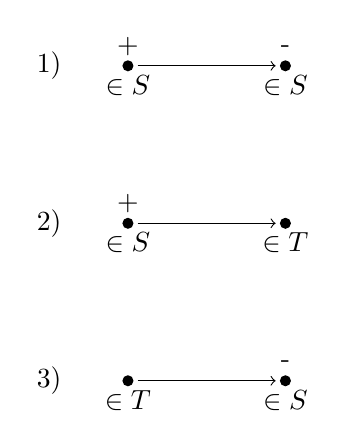
\begin{tikzpicture}
    \node (a0) at (0,0) {1)};
    \node (a1) at (1,0) {};
    \node (a2) at (3,0) {};
    \node (b0) at (0,-2) {2)};
    \node (b1) at (1,-2) {};
    \node (b2) at (3,-2) {};
    \node (c0) at (0,-4) {3)};
    \node (c1) at (1,-4) {};
    \node (c2) at (3,-4) {};
    
    \node at (1,0.25) {+};
    \node at (3,0.25) {-};
    \node at (1,-2 +0.25) {+};
    \node at (3,-4 +0.25) {-};
  
    \node at (1,-0.25) {$\in S$};
    \node at (3,-0.25) {$\in S$};
    \node at (1,-2.25) {$\in S$};
    \node at (3,-2.25) {$\in T$};
    \node at (1,-4.25) {$\in T$};
    \node at (3,-4.25) {$\in S$};
  
    \def\numone{1}
    \def\numtwo{2}
    \foreach \node in {a,b,c} 
    {
      \fill (\node\numone) circle(2pt);
      \fill (\node\numtwo) circle(2pt);
      \path (\node\numone) edge[->] (\node\numtwo);
    };
    
  \end{tikzpicture}
  \caption{3 possible cases}
\end{figure}
